\clearpage
\section{材质贴图的绿色与蓝色通道}
色板只有两个三角形。看左上角的红格，底色贴图把它涂成红色，另一张贴图决定它反光时的样子。glTF 将粗糙度放在这张材质贴图的绿色通道，将金属度放在蓝色通道。粗糙度越大，高光通常铺得越开。金属度为零对应塑料一类的绝缘体，为一对应金属。两项都是 $0$ 到 $1$ 之间的比例。

\begin{figure}[H]\centering
\newcommand{\channelsample}[1]{%
  \begin{tikzpicture}
    \node[anchor=south west,inner sep=0] (photo) at (0,0) {%
      \includegraphics[width=\linewidth,trim=183bp 37bp 183bp 37bp,clip]{../../../output/profiling/material-channels/#1.png}};
    \begin{scope}[x={(photo.south east)},y={(photo.north west)}]
      \draw[black,line width=1.55pt] (.295,.703) circle[radius=2pt];
      \draw[white,line width=.8pt] (.295,.703) circle[radius=2pt];
    \end{scope}
  \end{tikzpicture}}
\begin{minipage}[t]{.31\linewidth}\centering
\channelsample{albedo}\\[-1pt]
{\small\sffamily 底色}
\end{minipage}\hfill
\begin{minipage}[t]{.31\linewidth}\centering
\channelsample{roughness}\\[-1pt]
{\small\sffamily 粗糙度}
\end{minipage}\hfill
\begin{minipage}[t]{.31\linewidth}\centering
\channelsample{metallic}\\[-1pt]
{\small\sffamily 金属度}
\end{minipage}
\caption{RedflagForge 材质色板，RenderDoc 第 12 帧。圆圈标出同一个像素。从左向右看，它的底色偏红、粗糙度较低、金属度较高。后两张直接用灰度表示数值，越亮数值越大。}
\end{figure}

在材质贴图的同一位置，绿色通道存着 64，蓝色通道存着 255。两个数各占一个字节，除以 255 就能换成 $0$ 到 $1$ 的比例。模型文件给整块色板指定了粗糙度系数 $0.8$、金属度系数 $0.6$。将各自的系数乘进去，就能算出着色器应该读到什么。
\[
  \text{粗糙度}=0.8\,\frac{64}{255}\approx0.200784,\qquad
  \text{金属度}=0.6\,\frac{255}{255}=0.6 .
\]

\codewhere{着色器节选}{Redflag/src/Platform/Vulkan/Shaders/Mesh.frag}{main}
\begin{lstlisting}
vec2 material = unpackUnorm2x16(u_Object.MaterialFactors);
if ((u_Object.MaterialFlags & 4u) != 0u)  // (*@当前材质有这张贴图。@*)
    material *= texture(u_MetallicRoughnessMap, v_TexCoord).bg;
\end{lstlisting}

第一行取出本次绘制的两个系数。代码把金属度排在前面，所以 \code{.bg} 依次取蓝、绿通道。没有贴图时直接用系数。本页截帧时由着色器将底色从 sRGB 换为线性亮度，现版由 Vulkan 的 sRGB 纹理格式完成，末位精度可能不同。两版都按线性比例读取粗糙度和金属度。

在原图坐标 $(311,167)$ 读到粗糙度 $0.200733$，与手算相差约 $0.000052$。绘制时，两项材质各用 12 位保存，从 0 到 1 有 4095 个间隔，四舍五入最多差半个间隔，约 $0.000122$。这一点差别落在舍入误差之内。
\readings{\href{https://registry.khronos.org/glTF/specs/2.0/glTF-2.0.html\#metallic-roughness-material}{Khronos · glTF 2.0 §3.9.2}\quad
\src{Redflag/src/Platform/Vulkan/Shaders/MaterialChannels.glsl}{MaterialChannels.glsl · encodeMaterial}\quad
\href{run:../profiling/material-channels/samples.json}{四格原始读数}}

\clearpage
\section{色板上的法线}
色板第一次画出来时，中间有一条黑带。左上红格的粗糙度和金属度已经对上了，接着可以检查光照用到的方向。色板平放在 $xy$ 平面，正面朝向镜头，法线应沿 $+z$。从 RenderDoc 的绘制事件 27 读第二张输出图，却发现整个色板都沿 $+y$，像是把平面立错了方向。

\begin{figure}[H]\centering
\begin{minipage}[t]{.483\linewidth}\centering

\includegraphics[width=.68\linewidth,trim=183bp 37bp 183bp 37bp,clip]{../../../output/profiling/material-channels/panel-before.png}\hfill
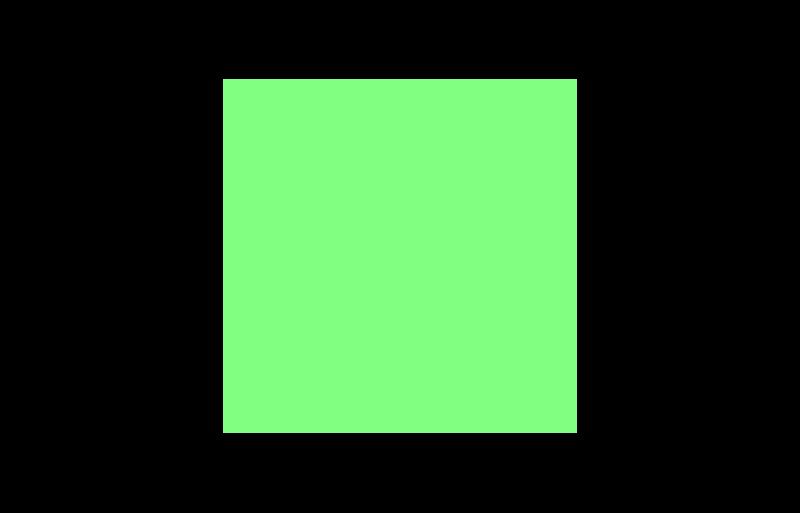
\includegraphics[width=.29\linewidth,trim=183bp 37bp 183bp 37bp,clip]{../../../output/profiling/material-channels/normal-before.png}\\
{\small\sffamily 修正前\quad 法线 $(0,1,0)$}
\end{minipage}\hfill
\begin{minipage}[t]{.483\linewidth}\centering
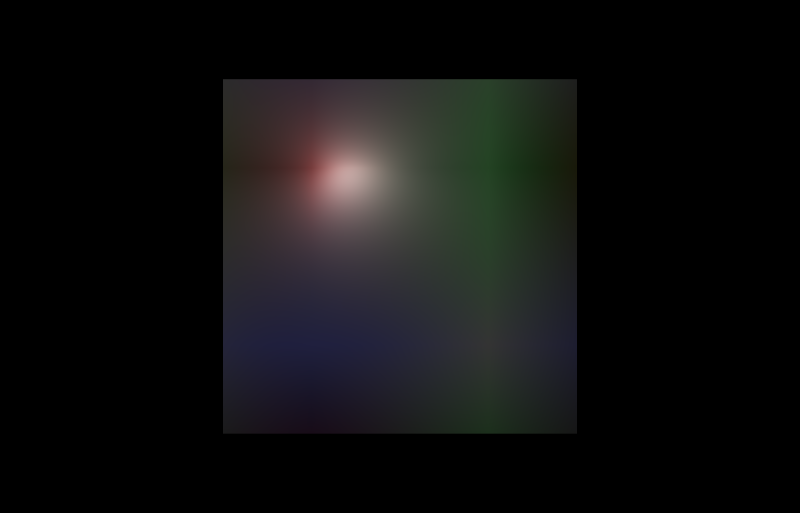
\includegraphics[width=.68\linewidth,trim=183bp 37bp 183bp 37bp,clip]{../../../output/profiling/material-channels/panel.png}\hfill
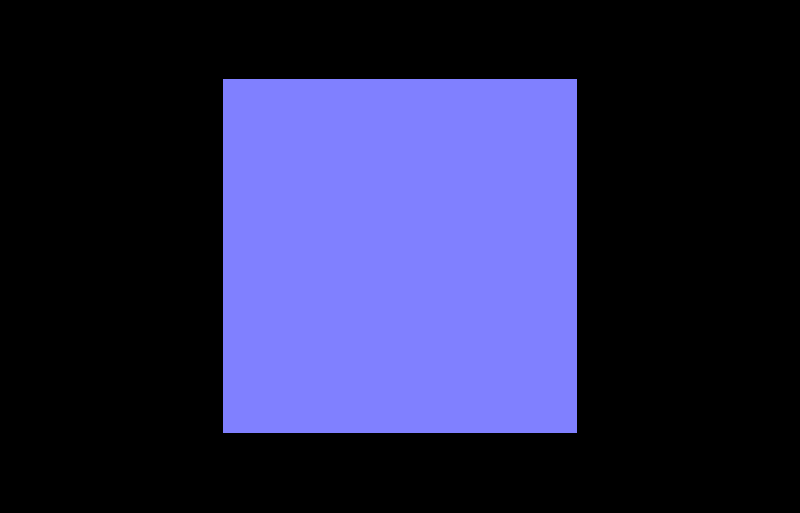
\includegraphics[width=.29\linewidth,trim=183bp 37bp 183bp 37bp,clip]{../../../output/profiling/material-channels/normal-after.png}\\
{\small\sffamily 修正后\quad 法线 $(0,0,1)$}
\end{minipage}
\caption{同机位两次 RenderDoc 回放。每组大图是场景面板，小图把世界法线的 $x,y,z$ 分别画成红、绿、蓝。修正后，高光出现在点光源照向的左上区域。两帧均覆盖 125,316 个模型像素。}
\end{figure}

色板文件给了顶点位置，省略了法线。取第一个三角形，从同一顶点沿两条边走，模型局部坐标中的边向量是 $(0,-4,0)$ 和 $(4,0,0)$。它们叉乘得到 $(0,0,16)$，除以长度 16 就是单位法线 $(0,0,1)$。glTF 约定缺少法线时按面计算，\code{Model::Load} 也已请求 \code{aiProcess\_GenNormals}。问题出在编译 Assimp 时关闭了这个步骤，模型最终读到了默认的朝上方向。

\codewhere{构建配置节选}{premake5.lua}{assimp}
\begin{lstlisting}
removedefines { "ASSIMP_BUILD_NO_GENFACENORMALS_PROCESS" }
files { "Redflag/vendor/assimp/code/GenFaceNormalsProcess.cpp" }
\end{lstlisting}

第一行解除对面法线生成器的禁用，第二行把它的实现编入项目。重新导入后，还可以用模型回归测试读取实际上传的三个顶点，分别检查法线是否等于预期方向。

回到同一帧，事件 39 将每个像素交给光照计算。一个表面用位置、法线和底色三个四分量向量保存，每个向量 16 字节，共 48 字节。位置的第四项标记这里有模型，法线的第四项保存粗糙度，底色的第四项保存金属度。在事件 27 还能查到整次绘制共用的压入常量（push constants）。拾取时存实体编号的 4 个字节，在材质绘制时存两个 16 位系数，因此整块仍为 128 字节。
\readings{\src{Redflag/src/Platform/Vulkan/Shaders/PackSurfaces.comp}{PackSurfaces.comp · main}\quad
\src{Redflag/src/Platform/Vulkan/VulkanDraw.cpp}{VulkanDraw.cpp · DrawIndexed}\quad
\href{run:../profiling/material-channels/README.md}{两份原帧与命令}\\
\href{https://registry.khronos.org/glTF/specs/2.0/glTF-2.0.html\#meshes}{glTF 2.0 §3.7.2.1 · 几何属性}\quad
\href{https://pbr-book.org/4ed/Shapes/Triangle_Meshes}{PBRT 第四版 §6.5 · 三角形网格}}
